\documentclass{article}
\title{ECE 370 -- Homework 3}
\usepackage[margin=1in]{geometry}
\usepackage{graphicx}
\usepackage{pdfpages}
\usepackage{fancyhdr}
\usepackage{enumitem}
\usepackage{pdfpages}
\usepackage{amsmath}
\usepackage{amssymb}
\usepackage{float}
\pagestyle{fancy}
\fancyhf{}
\fancyhead[L]{Gianni Avilan-Losee}
\fancyhead[C]{ECE 370}
\fancyhead[R]{Homework 3}
\fancyfoot[C]{\thepage}
\usepackage{microtype}
\usepackage{textcomp, gensymb}
\author{Gianni Avilan-Losee}
\setcounter{section}{1}
\begin{document}
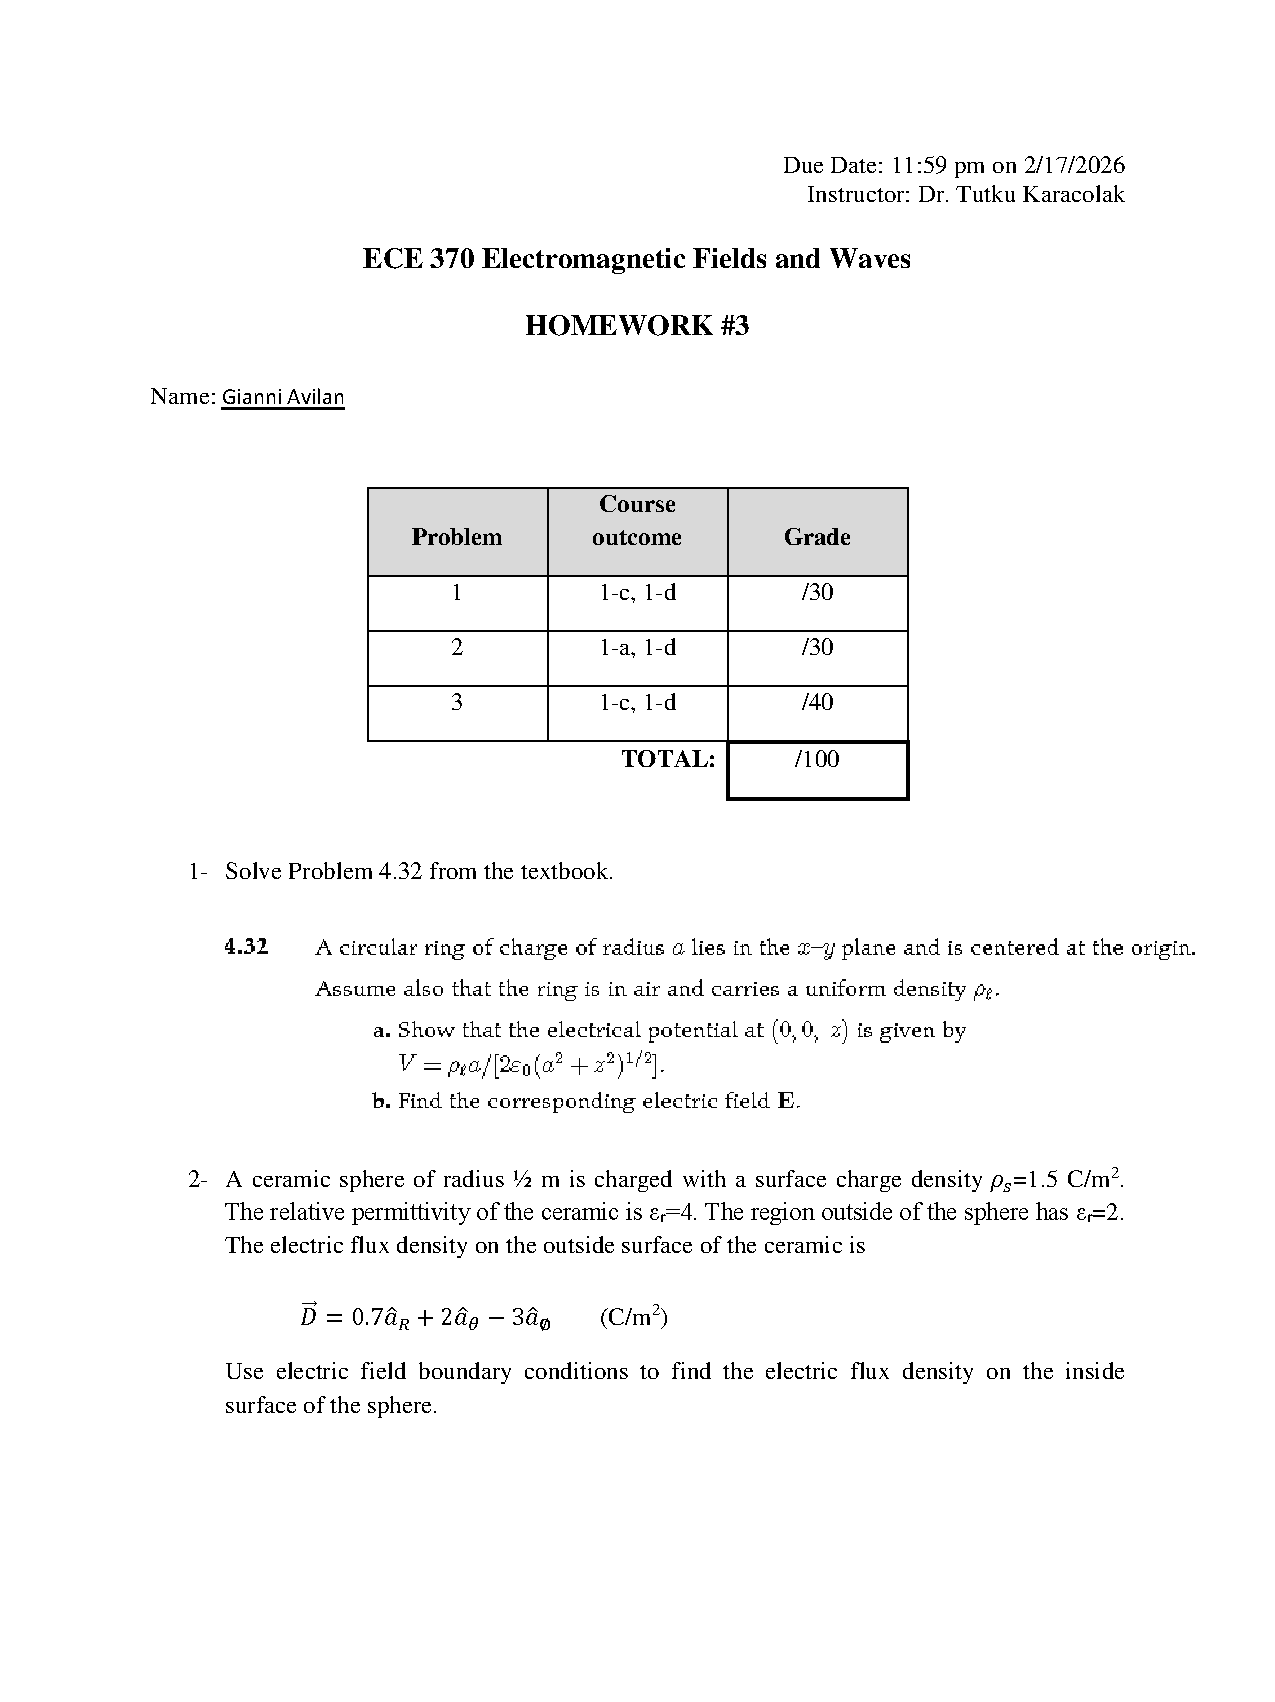
\includepdf[pages=-]{homework-3_cover-page.pdf}
\begin{enumerate}
	\item
		\begin{enumerate}[label=\alph*)]
			\item
				We may consider the given ring of charge to be a collection of infintesimal point charges, and find the electric potential at some point on the z-axis by summing the total effect of each point charge. 
				Here, we refer to \textbf{electric potential} as the difference in the potential energy of a unit charge (\(1\mathrm{C})\) at some point \(P\), with the implication that there is some quantifiable electric field intensity at \(P\), versus that same unit charge's potential energy infinitely far away from \(P\), with the implication that there is effectively no electric field at infinity.

				For a point charge with charge \(q\), this electric potential is given by \[
				  V = \frac{q}{4\pi\varepsilon|R-R_1|},
				\]
				with \(|R-R_1|\) representing the shortest distance between the point charge and \(P\). Since there is no directional component to electric potential, and it reduces to a scalar, we may use the superposition principle to find the total influence of any number of point charges on the electric potential at \(P\) as the sum of their influences. Factoring out constant terms, \[
				  V = \frac{1}{4\pi\varepsilon}\sum_{i=1}^{N}\frac{q_i}{|R-R_1|}.
				\]
		As mentioned earlier, we may reduce the given ring of charge of radius \(a\) to a collection of point charges \(q_i\), where each point charge carries a charge of \(\rho_\ell\). We will note that, by centering the ring of charge at the origin of the x-y axis, each of these infinitesimal point charges lies at an equal distance to any given point along the z-axis, so that for any one point charge, \(|R-R_1| = \sqrt{z^2 + a^2}\). Since this term is constant for any point \((0,0,z)\), we may now express the electric potential at \(z\) as \[
			\frac{1}{4\pi\varepsilon \sqrt{z^2 + a^2}} \sum_{i=1}^{N} \rho_{\ell} dl.
		\]
		We will also assume a permittivity of \(\varepsilon_0\), since the permittivity of air is virtually identical to free space permittivity.  Summing all point charges around the entire ring, we could derive the corresponding integral using cylindrical coordinates, or simply use the well-known formula for the circumference of a circle, \(2\pi R\), and reduce the formula for electric potential at \((0,0,z)\) to \[
			V_z = \frac{\rho_{\ell}2\pi a}{4\pi\varepsilon_0 \sqrt{z^2+a^2}} = \frac{\rho_\ell a}{2\varepsilon_0 \sqrt{z^2+a^2}} \ \mathrm{V}.
		\]
	\item Though we could use the methods from the previous homework, such as Gauss's Law, to derive the electric field \(\vec{E}\) at some point \((0,0,z)\), it is easier to use the electric potential itself to derive the electric field. We will use the relationship \[
	  \vec{E} = -\nabla V;
	\] 
	in other words, electric field is the gradient of electric potential, with its sign changed. 
	
	Finding electric field at \((0,0,z)\), noting that the electric potential on the z-axis does not depend on x or y, \[
		\vec{E}_z= -(\frac{\partial V_z}{\partial x}\hat{\alpha_x} + \frac{\partial V_z}{\partial y}\hat{\alpha_y} + \frac{\partial V_z}{\partial z}\hat{\alpha_z}) = -\frac{\partial V_z}{\partial z}\hat{\alpha_z} = -\frac{\rho_\ell a}{2\varepsilon_0}\frac{d}{dz}\frac{1}{\sqrt{z^2+a^2}} = \frac{\rho_{\ell}a z}{2\varepsilon_0(z^2+a^2)^{\frac{3}{2}}}\hat{\alpha_z} \ \mathrm{\frac{V}{m}} 
	\]
		\end{enumerate}
	\item Using boundary conditions, we know that the surface charge density at the boundary between two materials with differing relative permittivities is equal to the difference between the components of electric flux density normal to the boundary in each region.  Mathematically, \[
			D_{1n} - D_{2n} = \rho_s \Rightarrow D_{1n} = \rho_s + D_{2n}.
	\]
  Given surface charge density \(1.5\mathrm{\frac{C}{m^2}}\) and flux density normal to the outer boundary of the ceramic sphere of \(0.7\) (in spherical coordinates, all three unit vectors are mutually perpendicular, and so \(\hat{\alpha_\theta}\) and \(\hat{\alpha_\phi}\) define the plane tangent to the boundary's surface at any point), 
	\[
		D_{1n} = 1.5 + 0.7 = 2.2 \hat{\alpha_R}\mathrm{\frac{C}{m^2}} 
  \] 

	Then, finding flux density tangent to the outer surface, we may use the relationship between flux densities tangent to the boundary. Mathematically, \[
		\frac{D_{1t}}{\varepsilon_1} = \frac{D_{2t}}{\varepsilon_2} \Rightarrow D_{1t} = \frac{\varepsilon_1}{\varepsilon_2}D_{2t}.
	\]
	Given the components of \(\vec{D}_2\) tangent to the boundary, \(2 \hat{\alpha_{\theta}} - 3 \hat{\alpha_\phi}\), and permittivities of \(\varepsilon_1 = 4\), \(\varepsilon_2=2\), \[
		D_{2t} = \frac{4}{2}(2\hat{\alpha_\theta} - 3 \hat{\alpha_\phi}) = 4 \hat{\alpha_\theta} - 6 \hat{\alpha_\phi}.
	\]
	Combining the two components, \[
	  \vec{D}_1 = 2.2 \hat{\alpha_R} + 4 \hat{\alpha_\theta} - 6 \hat{\alpha_\phi}.
	\] 
\item 
	\begin{enumerate}[label=\alph*)]
		\item To find the vector electric field, we may use \[
		  \vec{E} = -\nabla V.
		\]
    Taking the partial derivative for each direction in the x-y-z plane, \[
			-(\frac{\partial V}{\partial dx}\hat{\alpha_x} + \frac{\partial V}{\partial dy}\hat{\alpha_y} + \frac{\partial V}{\partial dz}\hat{\alpha_z}) = [2xy(z^2+1)] \hat{\alpha_x} + [x^2(z^2+1)]\hat{\alpha_y} + [2x^yz] \hat{\alpha_z} \ \mathrm{\frac{V}{C}}.
    \]
	\item In free space, the electric flux density \(\vec{D} = \varepsilon_0 \vec{E}\), and so \[
			\vec{D} = \varepsilon_0 [2xy(z^2+1)] \hat{\alpha_x} + \varepsilon_0 [x^2(z^2+1)]\hat{\alpha_y} + \varepsilon_0 [2x^2yz] \hat{\alpha_z} \ \mathrm{\frac{C}{m^2}} 
	\]
\item Since the straight line path from \(A = (1,2,5)\) to \(B=(1,2,1)\) represents a change in \(z\) but no change in \(x=1\) or \(y=2\), we can simply evaluate the z-component at each point and integrate along \(dz\) as, \[
		V_{AB} = -\int_{z=1}^{z=5}4z \ dz = -(50-2) = -48 \ \mathrm{V}.
\]
	\end{enumerate}
\end{enumerate}
\end{document}
